%%%%%%%%%%%%%%%%%%%%%%%%%%%%%%%%%%%%%%%%%
% Beamer Presentation
% LaTeX Template
% Version 1.0 (10/11/12)
%
% This template has been downloaded from:
% http://www.LaTeXTemplates.com
%
% License:
% CC BY-NC-SA 3.0 (http://creativecommons.org/licenses/by-nc-sa/3.0/)
%
%%%%%%%%%%%%%%%%%%%%%%%%%%%%%%%%%%%%%%%%%

%----------------------------------------------------------------------------------------
%	PACKAGES AND THEMES
%----------------------------------------------------------------------------------------

\documentclass{beamer}

\mode<presentation> {

% The Beamer class comes with a number of default slide themes
% which change the colors and layouts of slides. Below this is a list
% of all the themes, uncomment each in turn to see what they look like.

%\usetheme{default}
%\usetheme{AnnArbor}
%\usetheme{Antibes}
%\usetheme{Bergen}
%\usetheme{Berkeley}
%\usetheme{Berlin}
%\usetheme{Boadilla}
%\usetheme{CambridgeUS}
%\usetheme{Copenhagen}
%\usetheme{Darmstadt}
%\usetheme{Dresden}
%\usetheme{Frankfurt}
%\usetheme{Goettingen}
%\usetheme{Hannover}
%\usetheme{Ilmenau}
%\usetheme{JuanLesPins}
%\usetheme{Luebeck}
\usetheme{Madrid}
%\usetheme{Malmoe}
%\usetheme{Marburg}
%\usetheme{Montpellier}
%\usetheme{PaloAlto}
%\usetheme{Pittsburgh}
%\usetheme{Rochester}
%\usetheme{Singapore}
%\usetheme{Szeged}
%\usetheme{Warsaw}

% As well as themes, the Beamer class has a number of color themes
% for any slide theme. Uncomment each of these in turn to see how it
% changes the colors of your current slide theme.

%\usecolortheme{albatross}
%\usecolortheme{beaver}
%\usecolortheme{beetle}
%\usecolortheme{crane}
%\usecolortheme{dolphin}
%\usecolortheme{dove}
%\usecolortheme{fly}
%\usecolortheme{lily}
%\usecolortheme{orchid}
%\usecolortheme{rose}
%\usecolortheme{seagull}
%\usecolortheme{seahorse}
%\usecolortheme{whale}
%\usecolortheme{wolverine}

%\setbeamertemplate{footline} % To remove the footer line in all slides uncomment this line
%\setbeamertemplate{footline}[page number] % To replace the footer line in all slides with a simple slide count uncomment this line

%\setbeamertemplate{navigation symbols}{} % To remove the navigation symbols from the bottom of all slides uncomment this line
}

\usepackage{graphicx} % Allows including images
\usepackage{booktabs} % Allows the use of \toprule, \midrule and \bottomrule in tables
\usepackage[utf8]{inputenc} %Accenti
\usepackage{algorithm,algorithmic} %pseudo
\usepackage[italian]{babel}
\usepackage{amsmath}

\graphicspath{ {./images/} } %Path delle immagini

\newcommand{\bigO}{\ensuremath{\mathcal{O}}} % O assintotica
\newcommand{\bigT}{\ensuremath{\Theta}} % Theta Assintotica

\renewcommand{\algorithmicforall}{\textbf{foreach}} %forall -> foreach

%----------------------------------------------------------------------------------------
%	TITLE PAGE
%----------------------------------------------------------------------------------------

\title[Two-dimensional Pattern Matching]{Approfondimento sul Pattern Matching 2D} % The short title appears at the bottom of every slide, the full title is only on the title page

\author{Liva Giovanni} % Your name
\institute[Udine] % Your institution as it will appear on the bottom of every slide, may be shorthand to save space
{
Università di Udine \\ % Your institution for the title page
\medskip
%\textit{liva.giovanni@spes.uniud.it} % Your email address
}
\date{\today} % Date, can be changed to a custom date

\begin{document}

\begin{frame}
\titlepage % Print the title page as the first slide
\end{frame}

\begin{frame}
\frametitle{Argomenti} % Table of contents slide, comment this block out to remove it
\tableofcontents % Throughout your presentation, if you choose to use \section{} and \subsection{} commands, these will automatically be printed on this slide as an overview of your presentation
\end{frame}

%----------------------------------------------------------------------------------------
%	DEBUG SLIDES
%----------------------------------------------------------------------------------------

\section{Lavori Precedendi}
\begin{frame}
\frametitle{Definizioni di Base}

\begin{definition}
\begin{itemize}
	\item $P$ viene usato per indicare un pattern unidimensionale di lunghezza $m$
	\item $T$ viene usato per indicare un testo unidimensionale di lunghezza $n$
	\item $PA$ viene usato per indicare un pattern bidimensionale di lunghezza $m\times m'$			\item $TA$ viene usato per indicare un testo bidimensionale di lunghezza $n \times n'$
	\item $D_H(x,y)$ è la funzione che calcola la distanza di hamming tra $x$ ed $y$
	\item $k$ viene usato per indicare il numero massimo di errorri ammessi
\end{itemize}	
\end{definition}
\end{frame}

\begin{frame}
\frametitle{Definizioni di Base}
\begin{figure}[p]
    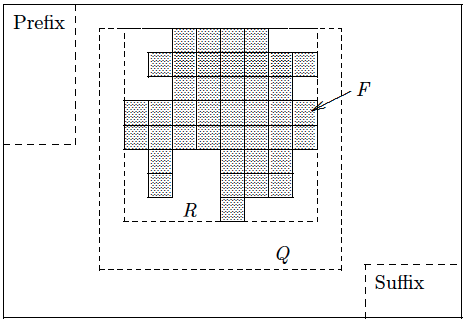
\includegraphics[width=0.6\textwidth]{def.png}
\end{figure}
\begin{definition}
	\begin{itemize}
		\item $F$ è un fattore 
		\item $R$ è l'array di contenimento (minimo), così come $Q$
	\end{itemize}	
\end{definition}
\end{frame}

\subsection{Exact vs Approximate}

%21
\begin{frame}
\frametitle{Exact vs Approximate}
Il pattern matching esatto prevede di cercare l'occorrenza di una stringa all'interno di un testo.
L'uso di automi per questo approccio è abbastanza naturale come si vede dal seguente algoritmo:\\
\begin{algorithm}[H]
\begin{algorithmic}[1]

\STATE $\delta(q_0,a) = \{q_0\} , \forall a \in A$\\

%\STATE $\delta(q_0,p_1) = \{q_0,q_1\}$\\

\FOR{$i=0$ to $m$}

\STATE $\delta(q_i,p_{i}) = \{q_{i+1}\}$

\ENDFOR
\end{algorithmic}
\caption{Creazione FA :: Pattern - Matching Esatto}
\end{algorithm}

L'automa risultante ha $m+1$ stati. Ogni stato $q_i$ indica che si è letto il prefisso del pattern fino all'$i$-esimo carattere

\end{frame}

\begin{frame}
\frametitle{Exact vs Approximate}

Il pattern matching approsimato si basa sulla distanza di Hamming che permette di quantificare il numero di errori ammessi.
La costruzione di tale automa prevede l'uso di $k+1$ copie di automi per il Pattern Matchin esatto, $M_0,\dots ,M_k$. \\
L'idea è quella che ogni $M_i$ rappresenta il pattern accettato con $i$ errori.
I vari $M_i$ sono collegati con una transizione dallo stato $q_j$ allo stato $q_{j+1}$ che corrisponde all'azione di $sostituzione$ nel calcolo della distanza di Hamming, etichettata con il simbolo $\overline{p}_{j+1}$ corrispondente al carattere complementare in posizione $j+1$ in P.\\

\end{frame}

\begin{frame}
\frametitle{Exact vs Approximate}
\setbeamercolor{block title}{use=structure,fg=white,bg=red!75!black}
  \setbeamercolor{block body}{use=structure,fg=black,bg=red!20!white}
\begin{theorem}[]
L'automa per il Pattern Matching approsimato ha $(k+1)(m+1 - k/2)$ stati
\end{theorem}

\begin{figure}[p]
    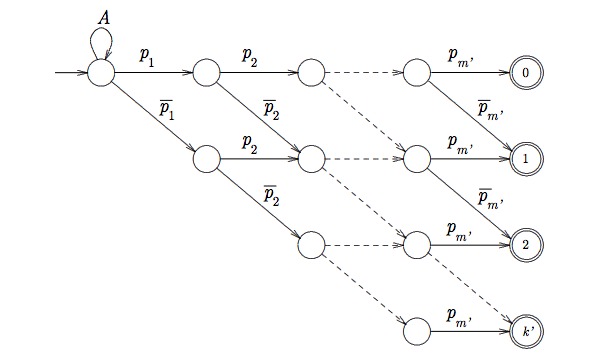
\includegraphics[scale=0.4]{approssimato.png}
\end{figure}

%\setbeamercolor{block title}{use=structure,fg=white,bg=green!35!black}
 % \setbeamercolor{block body}{use=structure,fg=black,bg=green!20!white}
%\begin{proof}
%
%\end{proof}

\end{frame}

\subsection{Approximate Dictionary Matching}
%22
\begin{frame}
\frametitle{Approximate Dictionary Matching}

\begin{definition}
	Sia $\pi$ un dizionario di $s$ pattern, $\pi = \{p_1,\dots,p_s\}$\\
	Sia $m = min\{|p_1|,\dots,|p_s|\}$\\
	Sia $k$ il numero di errori ammessi per ogni pattern, $k < m$ \\
	L'automa $\mathcal{A}$ per l'approximate dictionary matching riconosce il linguaggio $L(\mathcal{A}) =\bigcup_{i=1}^s \{ uv | u,v\in A^*, D_H(p_i,v) \leq k, p_i\in \pi \}$
\end{definition}

\begin{algorithm}[H]
\begin{algorithmic}[1]
\algsetup{linenosize=\tiny}
  \scriptsize
\FOR{$i=1$ to $s$}

\STATE Costruisci $M_i$ con la tecnica per il pattern matching approssimato

\ENDFOR
\STATE Costruisci lo stato iniziale $q_0$
\STATE $\delta(q_o,a) = \{q_0^i\} \forall a\in A, \forall i \in \{0,\dots,s\}$
\FOR{$i=1$ to $s$}
\STATE Aggiungi una transizione da  $q_0$ a $q_1^i$ etichettata come la transizione $q_0^i \to q_1^i$
\ENDFOR

\end{algorithmic}
\caption{Creazione FA :: Approximate Dictionary Matching}
\end{algorithm}

\end{frame}



\subsection{Baker and Bird}
%31
\begin{frame}
\frametitle{Baker and Bird}
\begin{definition}
	Sia $\pi$ il dizionario ottenuto da PA, $\pi= \{p_i | p_i \text{ è la } i \text{-esima colonna di PA}\}$\\
	Sia $\mathcal{A}$ l'automa ottenuto da PA con l'algoritmo di $Aho-Corasick$\\
	Sia $TA'$ il $text array$ ottenuto lanciando $\mathcal{A}$ su ogni colonna di TA e salvando lo stato corrente della run dell'automa
\end{definition}

\begin{itemize}
\item Linearizzare $TA'$ ottenendo $T$
\item Linearizzare $PA$ ottenendo $P$
\item Usare KMP su P e T
\item La complessità finale è  \bigO{$(mm' + nn')$} 
\end{itemize}


\end{frame}

\begin{frame}
\frametitle{Esempio}

\begin{figure}[p]
    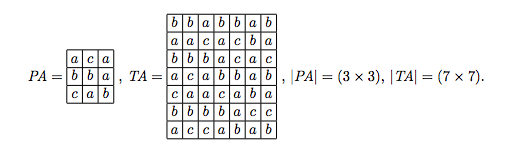
\includegraphics[width=0.5\textwidth]{Baker_Bird_1.png}
\end{figure}
\end{frame}

\begin{frame}
\frametitle{Esempio}

\begin{figure}[p]
    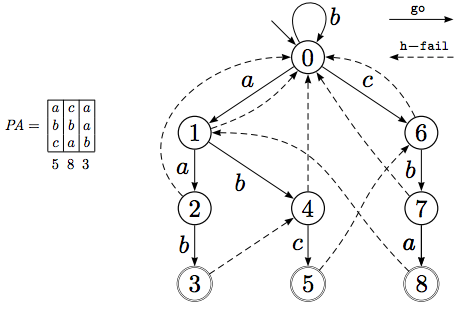
\includegraphics[width=0.5\textwidth]{Baker_Bird_2.png}
\end{figure}
\end{frame}

\begin{frame}
\frametitle{Esempio}

\begin{figure}[p]
    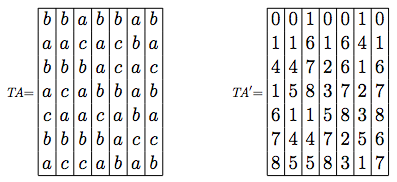
\includegraphics[width=0.5\textwidth]{Baker_Bird_3.png}
\end{figure}
\end{frame}

\begin{frame}
\frametitle{Esempio}

\begin{figure}[p]
    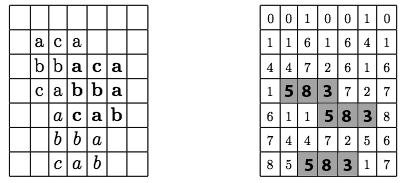
\includegraphics[width=0.4\textwidth]{Baker_Bird_4.png}
\end{figure}
\end{frame}

\subsection{Zhu and Takaoka}
%34
\begin{frame}
\frametitle{Zhu and Takaoka}

Estende l'idea di Karp e Rabin alle due dimensioni usando la tecnica delle $impronte$.\\
I passi dell'algoritmo sono:
\begin{itemize}
\item Genera $P'$ come array di impronte di PA usando la funzione di hash per colonne
\item Genera $T'$ nello stesso modo di $P'$ (Guardando solo $m'$ caratteri per colonna di TA)
\item Lancia KMP su $P'$ e$T'$ e ogni volta che trova una occorrenza esegue il controllo sulle matrici
\item Passa alla riga successiva aggiornando $T'$
\end{itemize}

Nel caso pessimo la complessità è $\bigO{(n'n + n'mm')}$

\end{frame}


\section{2D con FA}

\begin{frame}
\frametitle{2D con Finite Automata}
\Huge{\centerline{2D con Finite Automata}}
\end{frame}

%\subsection{Algo Generico}
%40
\begin{frame}
\frametitle{2D Approsimato con FA :: Algoritmo Generico}
\begin{definition}
	Sia $\pi$ il dizionario ottenuto da PA, $\pi= \{p_i | p_i \text{ è la } i \text{-esima colonna di PA}\}$\\
	Sia $R$ la linearizzazione di PA\\
	Sia $M(\pi) = (Q,A,\delta,I,F)$ l'automa costruito con la tecnica per l'approximate dictionary matching\\
\end{definition}
\begin{itemize}
\item Costruiamo $M(\pi)$ con $k'$ errori 
\item Costruiamo $TA'$ ottenuto dai valori della run di $M(\pi)$ su TA
\item Costruiamo $R$ come l'insieme degli stati finali di $M(\pi)$ che rappresentano il match esatto di PA
\item Costruiamo $M'$ che cerca $R$ con $k$ errori (limitiamo la somma degli errori del punto 1)
\item Lanciamo $M'$ su $TA'$ in modo che rilevi tutte le occorrenze di $R$
\end{itemize}

\end{frame}
%\subsection{2D Esatto}
%41
%\subsection{BlowUp state explosion Problem}
%44
%\subsection{2D Con Errori}
%47
%\subsection{Pratical 2D PM con Hamming}
%53
\begin{frame}
\frametitle{Caso Esatto :: Costruzione $M(\pi)$}

$M(\pi)$ riconosce il linguaggio $L = A*E(\pi)$ con $E(\pi) = \{ P \in A^{m'} ; P \in \pi   \}$\\
La costruzione di tale automa consiste in un $Trie$ con un self loop sullo stato iniziale etichettato con $A$ e $m$ transizioni verso gli automi per i singoli pattern.

\begin{figure}[p]
    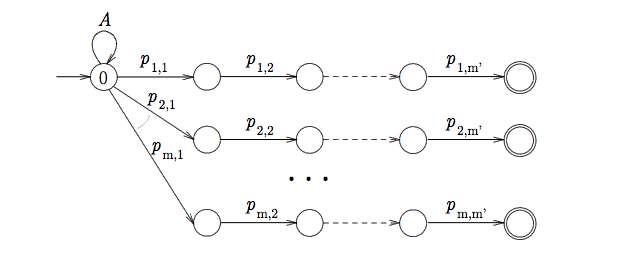
\includegraphics[width=0.8\textwidth]{exact2D.png}
\end{figure}

\end{frame}

\begin{frame}
\frametitle{Caso Esatto :: Costruzione $M(\pi)$}

\setbeamercolor{block title}{use=structure,fg=white,bg=red!75!black}
  \setbeamercolor{block body}{use=structure,fg=black,bg=red!20!white}
\begin{theorem}[]
L'automa ha al più uno stato finale attivo dopo aver letto un carattere d'input.
\end{theorem}


\setbeamercolor{block title}{use=structure,fg=white,bg=green!35!black}
  \setbeamercolor{block body}{use=structure,fg=black,bg=green!20!white}
\begin{proof}
Siccome $\pi$ è un insieme, non esistono duplicati di una stringa.\\
Visto che ogni stringa all'interno di $\pi$ ha la stessa lunghezza, dopo ogni step dell'automa solo, al più, uno stato finale può essere attivo.
\end{proof}
Questo teorema vale grazie a come viene eseguita la simulazione di $M(\pi)$.

\end{frame}

\begin{frame}
\frametitle{Caso Esatto :: Costruzione $TA'$}
Grazie al teorema precedente possiamo costruire $TA'$ usando la seguente formula:
\begin{equation*}
\forall  i,j\ 1\leq i \leq n, 1 \leq j \leq n'\
TA'[i,j]= 
\begin{cases} q & \text{se $q\in F$}
\\
0 &\text{se $q \not\in F$}
\end{cases}
\end{equation*}


\end{frame}

\begin{frame}
\frametitle{Caso Esatto :: Costruzione $R$}
La stringa $R$ è ottenuta linearizzando PA grazie all'automa $M(\pi)$ costruito in precedenza.\\
L'$i$-esimo carattere di $R$ è ottenuto leggendo lo stato finale di $M(\pi)$ su input PA[$i$]. \\


\end{frame}

\begin{frame}
\frametitle{Caso Esatto :: Costruzione $M'$}
Costruiamo l'automa $M'$ con il solito algoritmo sull'alfabeto $F \cup \{0\}$ che riconosca il linguaggio $L(M') = (F \cup \{0\}) * E(R)$ dove $E(R) =  \{R\ |\ R \in F^m\} $, $F = \{s1,\dots,s_{|\pi|}\}$, $|F| = |\pi|$.
\begin{figure}[p]
    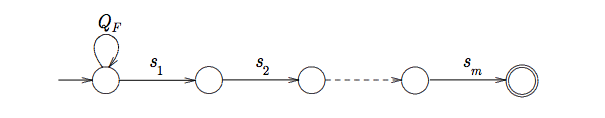
\includegraphics[width=0.8\textwidth]{exact2D_m1.png}
\end{figure}

\end{frame}

\begin{frame}
\frametitle{Caso Esatto :: Conclusioni}
\begin{itemize}
\item Tutti gli automi presentati sono non deterministici
\item Bisogna utilizzare una simulazione per non dover determinizzare gli automi
\item Opera in tempo lineare: $\bigO{(mm'+nn')}$
	\begin{itemize}
	\item $\bigO{(mm')}$ per $M(\pi)$
	\item $\bigO{(nn')}$ per $TA'$
	\item $\bigO{(m)}$ per $R$ ed $M'$
	\item $\bigO{(nn')}$ per il pattern matching
	\end{itemize}
\end{itemize}
\end{frame}


\begin{frame}
\frametitle{Caso Approssimato}
Dobbiamo modificare $M(\pi)$ in modo che accetti il linguaggio $L(M) = A * H_k(\pi)$ dove: $H_k(\pi) = \{X\ |\ X \in A^*, D_H(X,P) \leq min(k,m'-1) \wedge P\in \pi \}$\\
Dobbiamo usare il minimo perchè $k$ potrebbe essere più grande della dimensione di una colonna/righa.\\
Bisogna costruire l'automa per l'Approximate Dictionary Matching con l'algoritmo visto in precedenza con una modifica, gli stati finali sono etichettati con copie $(s,x)$ dove:
\begin{itemize}
\item $s$ = l'indice del pattern riconosciuto
\item $x$ = il numero di errori con il quale viene riconosciuto
\end{itemize}
\end{frame}

\begin{frame}
\frametitle{I singoli automi del ADM}
\begin{figure}[p]
    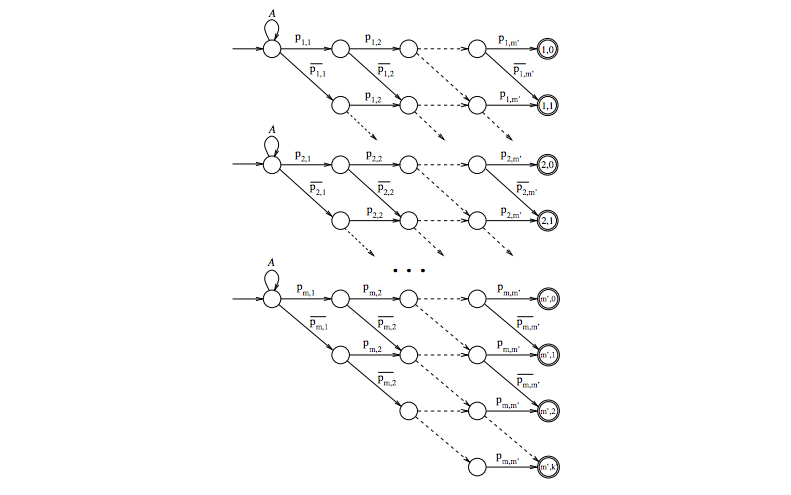
\includegraphics[width=1\textwidth]{ADM.png}
\end{figure}

\end{frame}

\begin{frame}

\begin{definition}
$k' = min(k, m'-1)$
\end{definition}

\frametitle{Caso Approssimato}
\setbeamercolor{block title}{use=structure,fg=white,bg=red!75!black}
  \setbeamercolor{block body}{use=structure,fg=black,bg=red!20!white}
  \begin{theorem}[]
  L'automa ha $|\pi|(k'+1)(m+1 - k'/2)$ stati di cui $|\pi|(k'+1)$ finali
  \end{theorem}
\begin{theorem}[]
L'automa potrebbe avere più di uno stato finale attivo dopo aver letto un carattere d'input.
\end{theorem}
\end{frame}


\begin{frame}
\frametitle{Caso Approssimato :: Costruzione $TA'$}
Dobbiamo estendere $TA'$ ad un array tridimensionale in quanto più pattern allo stesso istante potrebbero venire riconosciuti.\\
\begin{definition}
Sia $\oslash \not\in Q$ un simbolo nuovo che non appare negli stati e nelle label. \\
$\oslash$ viene usato per indicare che nessun pattern è trovato in una data posizione
\end{definition}

\begin{equation*}
\forall  i,j,s\ 1\leq i \leq n, 1 \leq j \leq n',1 \leq s \leq |\pi|
\end{equation*}
\begin{equation*}
TA'[i,j,s]= 
\begin{cases} 
x & \text{se $\exists q$ attivo, $q\in F, q = (s,x)$}
\\
\oslash  &\text{altrimenti}
\end{cases}
\end{equation*}
\end{frame}


\begin{frame}
\frametitle{Caso Approssimato :: Costruzione R}

Per costruire $R$ a partire da $PA$ vorremmo usare lo stesso algoritmo visto per il caso esatto.\\
Nel caso approssimato $M(\pi)$ ha più stati finali per ogni pattern $p \in \pi$, bisogna quindi apportare i seguenti aggiustamenti:
\begin{itemize}
\item Per ogni sottoautoma $M_i$ di $M(\pi)$ viene selezionato (arbritariamente) uno stato finale
\item Lo stato finale scelto è della forma (s,x) e per costruire $R$ guardiamo solo alla componente $s$
\end{itemize}

\end{frame}


\begin{frame}
\frametitle{Caso Approssimato :: Costruzione di $M'$ }

L'idea è quella di costruire $k+1$ copie dell'automa che riconosce $R$ in maniera esatta ($M_0,\dots,M_k$), dove ogni coppia è numerata e il suo indice permette di contare quanti errori sono stati compiuti.
\begin{definition}
Sia $M' = (Q',A',\delta',q_{0,0}', F')$ dove
	\begin{itemize}
		\item $A' = F \cup \{\oslash\}$
		\item $\delta' : Q' \times A' \to \mathcal{P}(Q')$
		\item $q_{i,j}$ stato $j$-esimo dell'automa $i$-esimo
	\end{itemize}
\end{definition}





\end{frame}

\begin{frame}
\frametitle{Caso Approssimato :: Costruzione di $M'$}
Ogni stato $q_{i,j}$ ha una transizione verso lo stato $q_{k,j+1} (\forall k . i \leq k \leq m')$ etichettata con $(p,z)$ dove: 
\begin{itemize}
\item $p$ indica l'$p$-esimo carattere di $R$ riconosciuto
\item $z$ indica il numero di errori che si commette eseguendo tale transizione
\end{itemize}

Per calcolare $z$ si utilizza la seguente funzione:

\begin{equation*}
|(s,x) - (t,y)|= 
\begin{cases} 
|x-y| & \text{$s = t$}
\\
m'  &\text{$((s,t) \vee (t,y)) = \oslash$}
\\
m'  &\text{$s \not= t $}
\end{cases}
\end{equation*}


\end{frame}

\begin{frame}
\frametitle{Caso Approssimato :: Costruzione di $M'$}

\begin{figure}[p]
\vspace*{-3cm}
    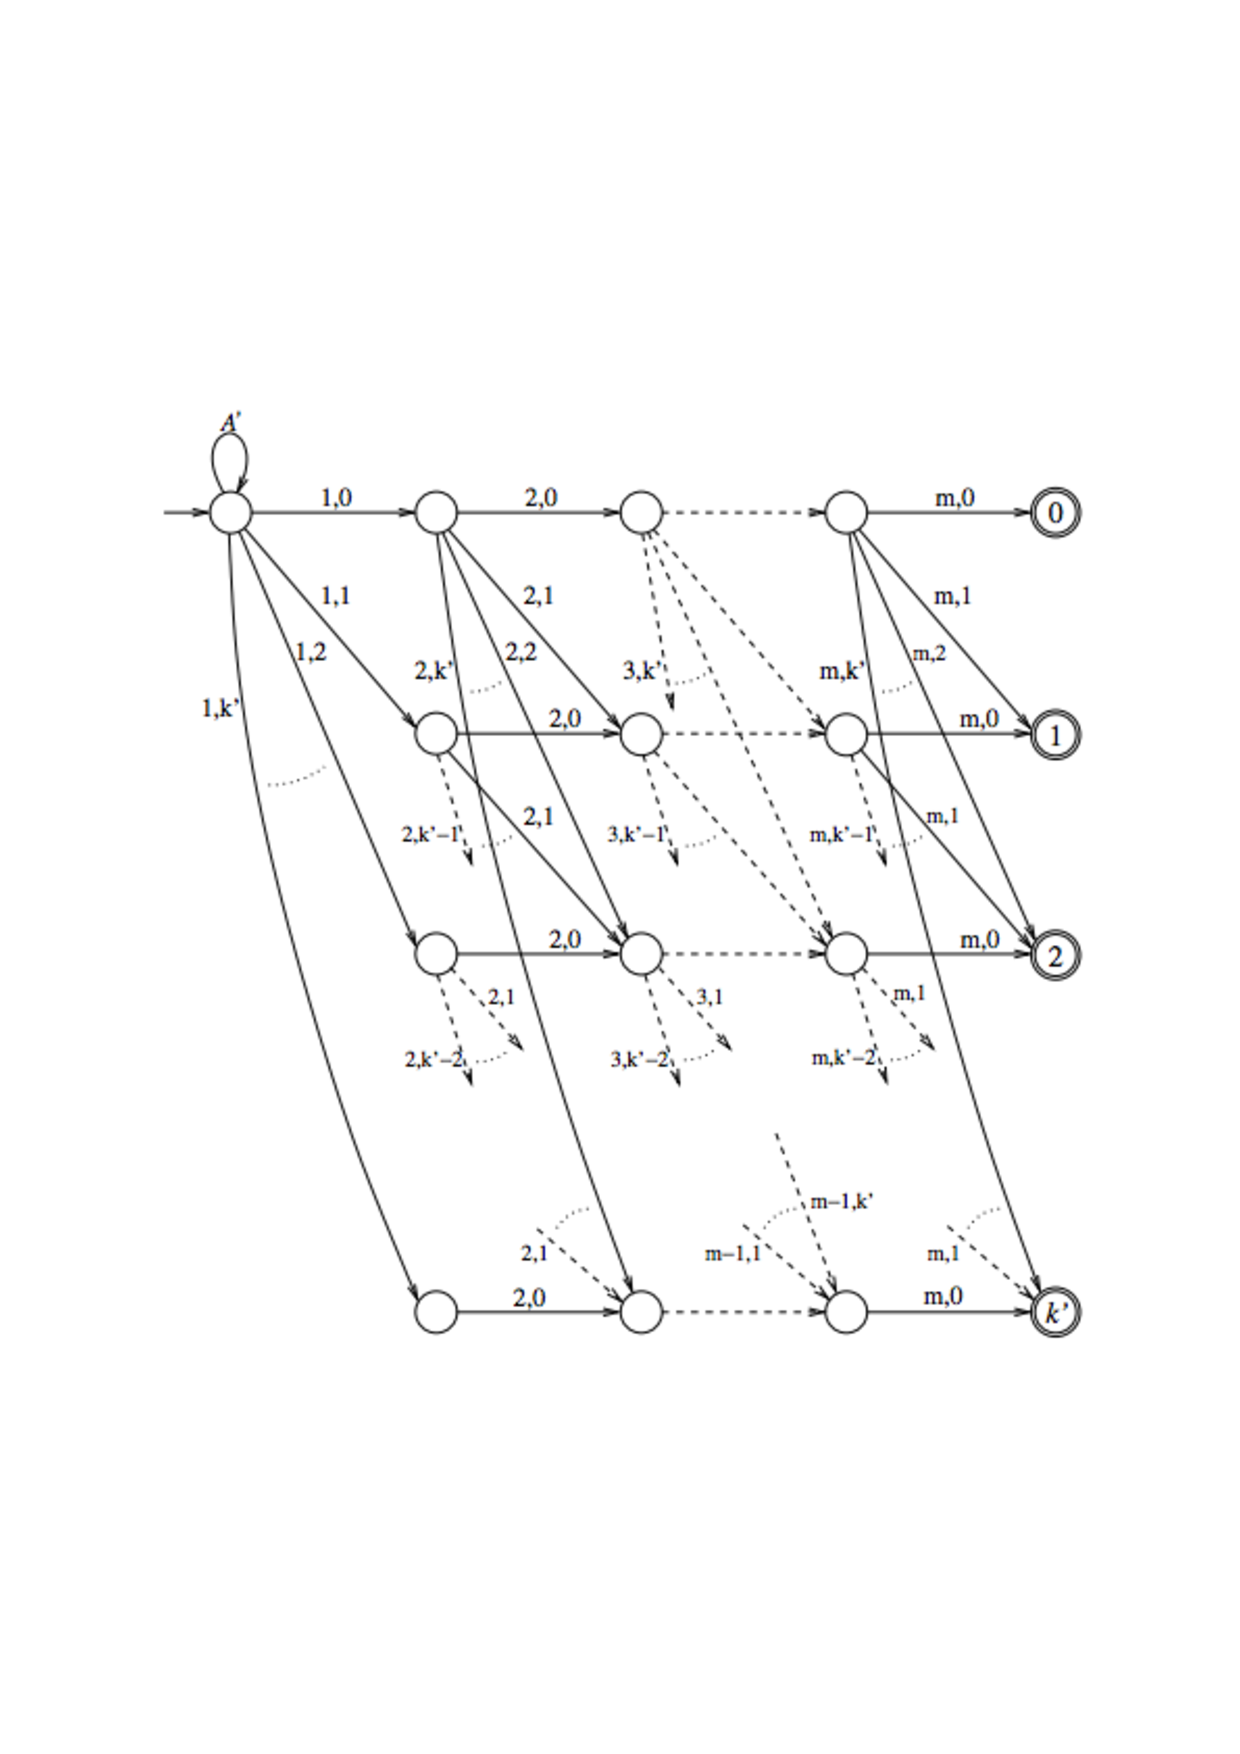
\includegraphics[width=0.8\textwidth]{aprox_count.pdf}
\end{figure}

\end{frame}

\begin{frame}
\frametitle{Simulazione}
Gli automi costruiti in questi passaggi sono non deterministici, la simulazione prevede l'uso della $programmazione$ $dinamica$.\\
Si introduce un array $E[0,\dots, m-1]$ che tiene conto del numero minimo di errori trovati.\\
Se uno stato attivo non compie nessuna transizione al passo successivo, questa computazione viene terminata.
\end{frame}


\begin{frame}

\begin{algorithm}[H]
\begin{algorithmic}[1]
\algsetup{linenosize=\tiny}
  \scriptsize
\FOR{$y=m'$ to $n'$}
\STATE $\forall q . E[q]$ inattivo
	\FOR{$x=1$ to $n$}
		\STATE E[0] attivo, E[0] = 0
		\FORALL{$q$ attivo in $E$}
			\STATE $err$ = $TA'[x,y,R[q+1]]$
			\IF{$err = \oslash$} \STATE $err = m'$ \ENDIF
			\STATE $err = err + E[q]$
			\IF {$err \leq k$} 
				\IF {$q+1 = m$} \STATE "Trovata Occorrenza"
				\ELSE \STATE $E[q+1]$ attivo, $E[q+1] = err$
				\ENDIF
			\ELSE \STATE $E[q+1]$ disattivato al prossimo step
			\ENDIF
		\ENDFOR
	\ENDFOR
\ENDFOR


\end{algorithmic}
\caption{Simulazione di $M'$ su $TA'$}
\end{algorithm}

\end{frame}

\begin{frame}
\frametitle{Conclusioni}

\begin{itemize}
\item $M(\pi)$ è fatto da $m$ sub-automi la cui simulazione su $TA$ richiede $m \cdot \bigO{(m'nn')}$
\item $R$ è costruito in $\bigO{(m)}$ 
\item La simulazione di $M'$ richiede $\bigO{(mnn' - mm'n)}$
\end{itemize}
La complessità totale dell'algoritmo per trovare PA in TA con $k$ errori chiede $\bigO{(mm' \cdot nn' + m +mnn' - mmn')} = \bigO{(mm' \cdot nn')}$

\end{frame}

\section{2D con PDA}
\begin{frame}
\frametitle{2D con PushDown Automata}
\Huge{\centerline{2D con PushDown Automata}}
\end{frame}
%\subsection{Img2Tree}

%\subsection{Indexing per space efficent}

%\subsection{Costruiamo il PDA}

\begin{frame}
\frametitle{Matrice Estesa}

\begin{definition}
Definiamo $A_\# = A \cup\{\#\}$ con $\#$ che non appare in $A$\\
Sia $M \in A^{(n\times n')}$, definiamo la matrice estesa $M' \in A_\# ^{(n+1 \times n'+1)}$ come $M$ con una nuova riga e colonna riempite con il carattere $\#$
\end{definition}

\[
  M = \begin{tabular} {|c|c|c|}
  	\hline
  		a & c & f  \\ 
  		\hline
  		b & e & h \\
  		\hline
  		d & g & i \\
  		\hline 
  \end{tabular} 
  \to M' = 
 \begin{array} {|c|c|c|c|}
 \hline
   		a & c & f & \# \\ 
   		\hline
   		b & e & h & \# \\
   		\hline
   		d & g & i  & \# \\
   		\hline
   		\# & \# & \# & \#\\
		\hline
   \end{array} 
\]


\end{frame}

\begin{frame}
\frametitle{Da matrice a DAG}

Dalla matrice $M'$ estesa possiamo creare un $DAG$ seguento le seguenti regole:
\begin{itemize}
\item La radice è in $M'[1,1] = M[1,1]$
\item Ogni nodo interno è formato dai valori di $M$
\item I caratteri $\# $ sono tutte foglie
\item Se un nodo $M'[i,j]$ è interno, allora ha due figli: $M'[i+1,j]$ e $M'[i,j+1]$
\end{itemize}

\begin{figure}[p]
    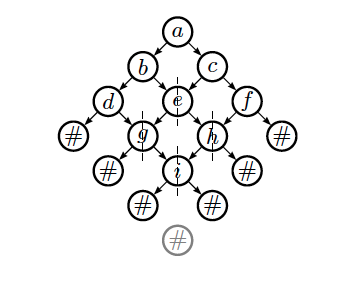
\includegraphics[width=0.5\textwidth]{dag.png}
\end{figure}
\end{frame}

\begin{frame}
\frametitle{Da DAG ad Albero}
La radice dell'albero è la radice del DAG.\\
In ricorsione si vedono i figli di un nodo e li si copiano nell'albero. Terminiamo quando arriviamo al nodo $\#$
\begin{figure}[p]
    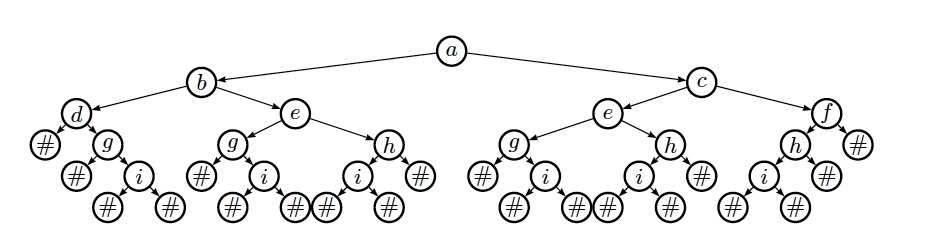
\includegraphics[width=1\textwidth]{tree.png}
\end{figure}


\end{frame}

\begin{frame}
\frametitle{Da Matrice ad Alberi}
Possiamo costruire direttamente l'albero a partire dalla matrice.\\
La struttura di DAG è mantenuta implicitamente.\\
\fontsize{10pt}{7.2}\selectfont
\[
	tree(M,x,y) = \begin{cases}
		(M[x,y], tree(M,x,y+1) , tree(M,x+1,y) ) & \text{Se $M[x,y] \not = \#$ }\\
		(M[x,y], null, null) & \text{Altrimenti}
	\end{cases}
\]
\fontsize{12pt}{7.2}\selectfont
\begin{definition}
Gli elementi della matrice che vengono visti più di una volta sono detti $splitting$ $nodes$.\\
$pref(t)$ è la visita in preorder con la stampa delle label dei nodi.
\end{definition}

\end{frame}

\begin{frame}
\frametitle{Index-Tree :: Da Alberi a DAG}
Notiamo che sottoalberi sono ripetuti più volte, possiamo allora eseguire una facile ottimizzazione.
\begin{figure}[p]
    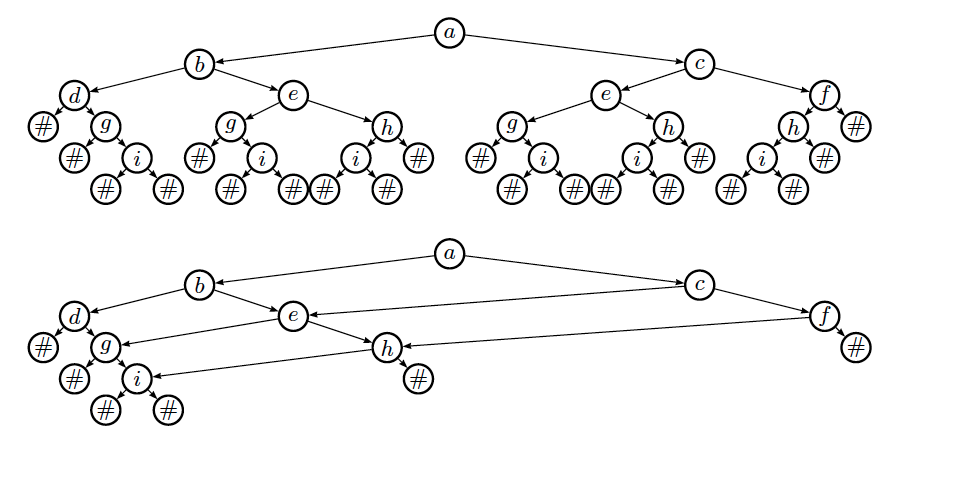
\includegraphics[width=1\textwidth]{index.png}
\end{figure}
\end{frame}

\begin{frame}
\frametitle{Da Matrice ad Alberi}
\setbeamercolor{block title}{use=structure,fg=white,bg=red!75!black}
  \setbeamercolor{block body}{use=structure,fg=black,bg=red!20!white}
\begin{theorem}[]
Sia $t$ ottenuto da $tree(M',1,1)$. La profondità massima di un nodo in $t$, $depth(t)$ è $depth(t) = n + n' -1$. 
\end{theorem}


\setbeamercolor{block title}{use=structure,fg=white,bg=green!35!black}
  \setbeamercolor{block body}{use=structure,fg=black,bg=green!20!white}
\begin{proof}
Il percorso più lungo in $t$ è quello che percorre $n -1$ nodi che non sono di $splitting$ e $n$ $splitting$ nodes.
\end{proof}

\frametitle{Da Matrice ad Alberi}
\setbeamercolor{block title}{use=structure,fg=white,bg=red!75!black}
  \setbeamercolor{block body}{use=structure,fg=black,bg=red!20!white}
\begin{theorem}[]
La costruzione dell'albero ha complessità $\bigO{(2^{depth(t)})}$
\end{theorem}


\setbeamercolor{block title}{use=structure,fg=white,bg=green!35!black}
  \setbeamercolor{block body}{use=structure,fg=black,bg=green!20!white}
\begin{proof}
In un albero binario completo il numero di nodi è $2^{depth(t)-1} + 2^{depth(t)} = \bigO{(2^{depth(t)})}$. 
\end{proof}
\end{frame}

\begin{frame}
\frametitle{Algoritmo Generico}
\begin{itemize}
\item Estendiamo il testo 2D e il pattern 2D 
\item \textbf{Costruiamo l'index del testo 2D come un PDA}
\item Costruiamo l'albero per il pattern 2D
\item \textbf{Linearizziamo il pattern calcolando $pref$ dell'albero}
\item \textbf{Cerchiamo il $pref$ del pattern con il PDA costruito al passo precedente}
\end{itemize}
\end{frame}

\begin{frame}
\frametitle{Algoritmo per la costruzione del PDA}
\begin{algorithm}[H]
\begin{algorithmic}[1]
	\STATE $\delta = \emptyset, Q = \emptyset, G = \{S\}$
	\STATE $G = G \cup \{S_{x+1,y}\}$ $\forall x,y\ 1\leq x < n \wedge 1 \leq y < n'$
	\STATE crea\_nodi()
	\STATE crea\_transizioni\_base()
	\STATE crea\_transizioni\_sharp()
	\STATE crea\_transizioni\_bottom()
	\STATE crea\_transizioni\_right()
	\STATE crea\_transizioni\_suffix()
	\STATE crea\_transizioni\_prefix()
\end{algorithmic}
\caption{Costruzione del PDA $\mathcal{M} = (Q,A_\#,G,\delta,q_{1,1},S,\emptyset)$}
\end{algorithm}

\end{frame}

\begin{frame}
\frametitle{Algoritmo per la costruzione del PDA}
\begin{algorithm}[H]
\begin{algorithmic}[1]
	\STATE $Q = Q \cup \{Q_{x,y}\}\ \forall x,y\ 1 \leq x \leq n+1,1\leq y \leq n'+1$ e $y<n' \vee x < n$
\end{algorithmic}
\caption{crea\_nodi()}
\end{algorithm}

\begin{algorithm}[H]
\begin{algorithmic}[1]
	\STATE $\delta(q_{x,y},TA[x,y],S) = \delta(q_{x,y},TA[x,y],S) \cup \{(q_{x,y+1},S_{x+1,y}S)\}$
	\STATE $\forall x,y\ 1\leq x < n, 1\leq y < n'$
\end{algorithmic}
\caption{crea\_transizioni\_base()}
\end{algorithm}

\begin{algorithm}[H]
\begin{algorithmic}[1]
	\STATE $\delta(Q_{n,y},\#,S) = \delta(q_{n,y},\#,S) \cup \{(q_{n+1,y},\epsilon)\}\ \forall y 1 \leq y < n'$
	\STATE $\delta(Q_{x,n'},\#,S) = \delta(q_{x,n'},\#,S) \cup \{(q_{x,n'+1},\epsilon)\}\ \forall x 1 \leq y < n$
\end{algorithmic}
\caption{crea\_transizioni\_sharp()}
\end{algorithm}

\end{frame}


\begin{frame}
\frametitle{crea\_nodi + crea\_transizioni\_base + crea\_transizioni\_sharp}
\begin{figure}[p]
    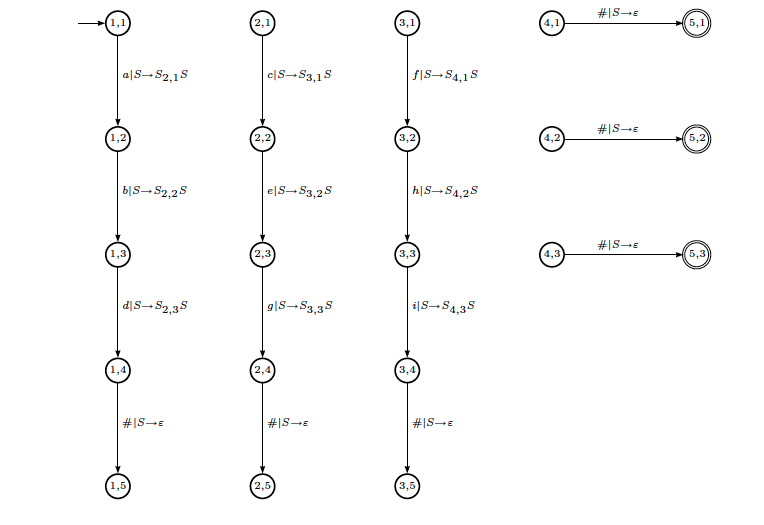
\includegraphics[width=1\textwidth]{pda_1.png}
\end{figure}
\end{frame}


\begin{frame}
\frametitle{Algoritmo per la costruzione del PDA}
\begin{algorithm}[H]
\begin{algorithmic}[1]
	\STATE $\delta(q_{x,n'+1},\epsilon,S_{x+1,y}) = \delta(q_{x,n'+1},\epsilon,S_{x+1,y}) \cup \{(q_{x+1,y},S)\}$
	\STATE  $\forall x,y$ $1 \leq x < n, 1\leq y < n'$
\end{algorithmic}
\caption{crea\_transizioni\_bottom()}
\end{algorithm}
\end{frame}


\begin{frame}
\frametitle{crea\_nodi + crea\_transizioni\_bottom}
\begin{figure}[p]
    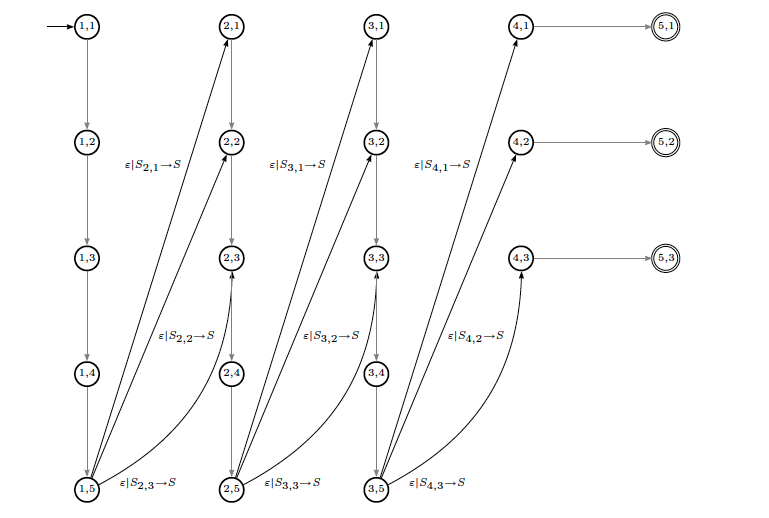
\includegraphics[width=1\textwidth]{pda_2.png}
\end{figure}
\end{frame}

\begin{frame}
\frametitle{Algoritmo per la costruzione del PDA}
\begin{algorithm}[H]
\begin{algorithmic}[1]
	\STATE $\delta(q_{n+1,y},\epsilon,S_{x,y-1}) = \delta(q_{n+1,y},\epsilon,S_{x,y-1}) \cup \{(q_{x,y-1},S)\}$
	\STATE  $\forall x,y$ $2 \leq x \leq n, 2\leq y < n'$
\end{algorithmic}
\caption{crea\_transizioni\_right()}
\end{algorithm}
\end{frame}


\begin{frame}
\frametitle{crea\_nodi + crea\_transizioni\_right}
\begin{figure}[p]
    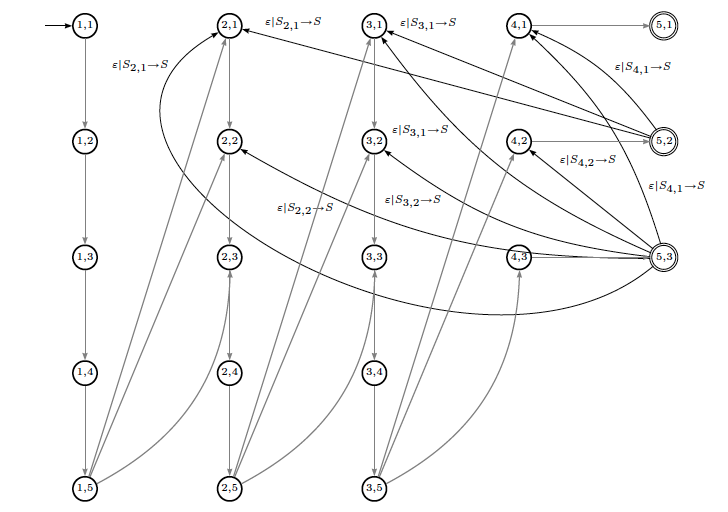
\includegraphics[width=1\textwidth]{pda_3.png}
\end{figure}
\end{frame}

\begin{frame}
\frametitle{nodi + basic + sharp + bottom + right}
\begin{figure}[p]
\vspace*{-0.35cm}
    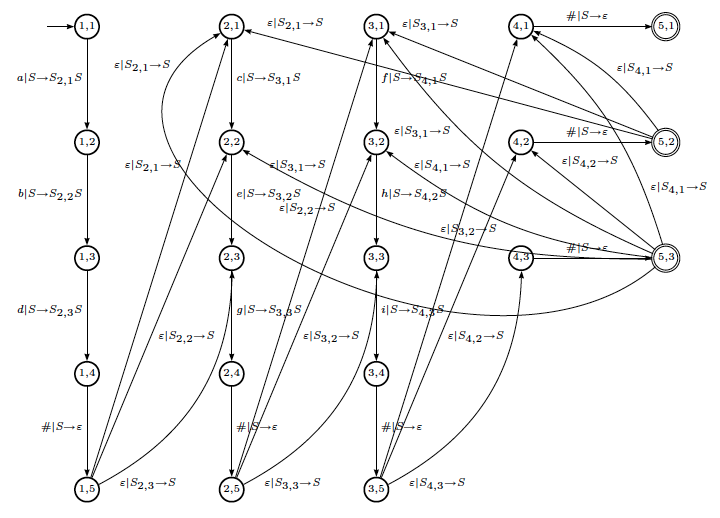
\includegraphics[width=0.95\textwidth]{pda_4.png}
\end{figure}
\end{frame}

\begin{frame}
\frametitle{Algoritmo per la costruzione del PDA}
\begin{algorithm}[H]
\begin{algorithmic}[1]
	\STATE $\delta(q_{1,1},TA[x,y],S) = \delta(q_{1,1},TA[x,y],S) \cup \{(q_{x,y+1},S_{x+1,y}S)\}$
	\STATE  $\forall x,y$ $1 \leq x < n, 1\leq y < n'$ e $x > 1 \vee y > 1$
\end{algorithmic}
\caption{crea\_transizioni\_suffix()}
\end{algorithm}

\begin{algorithm}[H]
\begin{algorithmic}[1]
	\STATE $\delta(q_{x,y},\#,S) = \delta(q_{x,y},\#,S) \cup \{(q_{n+1,y},\epsilon)\}$
	\STATE  $\forall x,y$ $1 \leq x < n, 1\leq y < n'$ e $x \not= 1 \vee y \not= 1$
\end{algorithmic}
\caption{crea\_transizioni\_prefix()}
\end{algorithm}

\end{frame}


\begin{frame}
\frametitle{nodi + suffix}
\begin{figure}[p]

    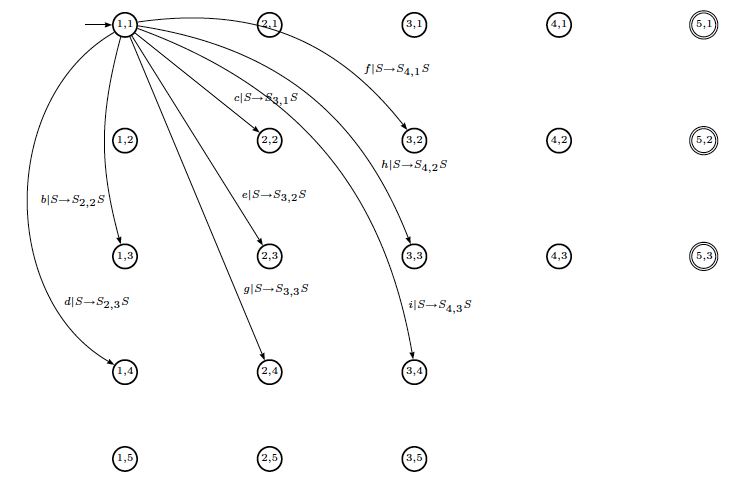
\includegraphics[width=0.95\textwidth]{pda_suf.png}
\end{figure}
\end{frame}

\begin{frame}
\frametitle{nodi + prefix}
\begin{figure}[p]
    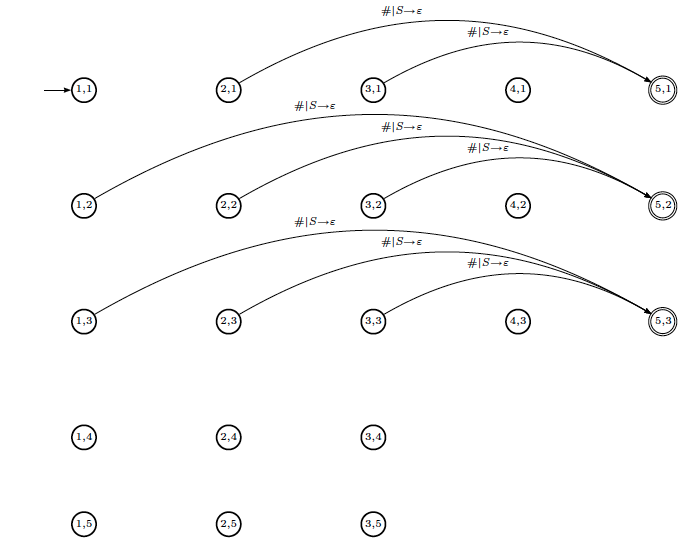
\includegraphics[width=0.85\textwidth]{pda_pre.png}
\end{figure}
\end{frame}

\begin{frame}
\frametitle{Dimostrazione correttezza}

\setbeamercolor{block title}{use=structure,fg=white,bg=red!75!black}
  \setbeamercolor{block body}{use=structure,fg=black,bg=red!20!white}
\begin{theorem}[]
Sia TA un testo 2D esteso. Il PDA $\mathcal{M}$ costruito da TA accetta tutti i $pref(F)$ con $F$ un fattore di TA. Quindi $\mathcal{M}$ accetta ogni $pref(TA[i..k,j..l]')$ con $1 \leq i \leq k \leq n, 1 \leq j \leq l \leq n'$
\end{theorem}


Dimostriamo per induzione sull'altezza dell'albero $t$ costruito con $tree(F,1,1)$:
\begin{itemize}
\item $F$ ha un solo elemento, $TA[i,j]$. $t$ ha altezza $1$ e $pref(t) = TA[i,j]\#\#$.\\
Per mezzo delle transizioni suffix: $(q_{i,j+1},S_{i+1,j}S) \in \delta(q_{1,1},TA[i,j],S)$\\
Quindi il PDA evolve nel seguente modo:\\
$(q_{1,1},TA[i,j]\#\#,S) \vdash_\mathcal{M}^+ (q_{n+1,j},\epsilon,\epsilon)$

\end{itemize}


\end{frame}

\begin{frame}
\frametitle{Dimostrazione correttezza}

\begin{itemize}
\item Assumiamo valga per $F_b = TA[i..k,j+1..l]$ e $F_r = TA[i+1..k,j..l]$. Sia $t_b = tree(F_b)$ e $t_r = tree(F_r)$ con $height(t_b) \leq m \wedge height(t_r) \leq m, m \geq 1$. Dimostriamo che vale anche per $t = TA[i,j]pref(t_b)pref(t_r), height(t) \geq m+1$\\
$(q_{1,1},TA[i,j]pref(t_b)pref(t_r),S) \vdash_\mathcal{M} $     \tiny{\%Leggiamo il primo carattere}\normalsize\\ %Leggiamo il primo carattere

$(q_{i,j+1},pref(t_b)pref(t_r),S_{i+1,j}S) \vdash_\mathcal{M}^+ $    \tiny{\%Per ip. Induttiva}\normalsize\\ %Ipotesi induttiva
$(q_{n+1,j+1},pref(t_r),S_{i+1,j}S) \vdash_\mathcal{M} $                   \tiny{\%Transizioni Right}\normalsize\\ %Suffix  
$(q_{i+1,j},pref(t_r),S) \vdash_\mathcal{M}^+ $                               \tiny{\%Per ip. Induttiva}\normalsize\\ %Ipotesi induttiva
$(q_{n+1,j},\epsilon,\epsilon)$.
\end{itemize}

\end{frame}


\begin{frame}
\frametitle{$\ $}
\Huge{\centerline{Fine}}
\end{frame}


%----------------------------------------------------------------------------------------
%	PRESENTATION SLIDES
%----------------------------------------------------------------------------------------

%%------------------------------------------------
%\section{First Section} % Sections can be created in order to organize your presentation into discrete blocks, all sections and subsections are automatically printed in the table of contents as an overview of the talk
%%------------------------------------------------
%
%\subsection{Subsection Example} % A subsection can be created just before a set of slides with a common theme to further break down your presentation into chunks
%
%\begin{frame}
%\frametitle{Paragraphs of Text}
%Sed iaculis dapibus gravida. Morbi sed tortor erat, nec interdum arcu. Sed id lorem lectus. Quisque viverra augue id sem ornare non aliquam nibh tristique. Aenean in ligula nisl. Nulla sed tellus ipsum. Donec vestibulum ligula non lorem vulputate fermentum accumsan neque mollis.\\~\\
%
%Sed diam enim, sagittis nec condimentum sit amet, ullamcorper sit amet libero. Aliquam vel dui orci, a porta odio. Nullam id suscipit ipsum. Aenean lobortis commodo sem, ut commodo leo gravida vitae. Pellentesque vehicula ante iaculis arcu pretium rutrum eget sit amet purus. Integer ornare nulla quis neque ultrices lobortis. Vestibulum ultrices tincidunt libero, quis commodo erat ullamcorper id.
%\end{frame}
%
%%------------------------------------------------
%
%\begin{frame}
%\frametitle{Bullet Points}
%\begin{itemize}
%\item Lorem ipsum dolor sit amet, consectetur adipiscing elit
%\item Aliquam blandit faucibus nisi, sit amet dapibus enim tempus eu
%\item Nulla commodo, erat quis gravida posuere, elit lacus lobortis est, quis porttitor odio mauris at libero
%\item Nam cursus est eget velit posuere pellentesque
%\item Vestibulum faucibus velit a augue condimentum quis convallis nulla gravida
%\end{itemize}
%\end{frame}
%
%%------------------------------------------------
%
%\begin{frame}
%\frametitle{Blocks of Highlighted Text}
%\begin{block}{Block 1}
%Lorem ipsum dolor sit amet, consectetur adipiscing elit. Integer lectus nisl, ultricies in feugiat rutrum, porttitor sit amet augue. Aliquam ut tortor mauris. Sed volutpat ante purus, quis accumsan dolor.
%\end{block}
%
%\begin{block}{Block 2}
%Pellentesque sed tellus purus. Class aptent taciti sociosqu ad litora torquent per conubia nostra, per inceptos himenaeos. Vestibulum quis magna at risus dictum tempor eu vitae velit.
%\end{block}
%
%\begin{block}{Block 3}
%Suspendisse tincidunt sagittis gravida. Curabitur condimentum, enim sed venenatis rutrum, ipsum neque consectetur orci, sed blandit justo nisi ac lacus.
%\end{block}
%\end{frame}
%
%%------------------------------------------------
%
%\begin{frame}
%\frametitle{Multiple Columns}
%\begin{columns}[c] % The "c" option specifies centered vertical alignment while the "t" option is used for top vertical alignment
%
%\column{.45\textwidth} % Left column and width
%\textbf{Heading}
%\begin{enumerate}
%\item Statement
%\item Explanation
%\item Example
%\end{enumerate}
%
%\column{.5\textwidth} % Right column and width
%Lorem ipsum dolor sit amet, consectetur adipiscing elit. Integer lectus nisl, ultricies in feugiat rutrum, porttitor sit amet augue. Aliquam ut tortor mauris. Sed volutpat ante purus, quis accumsan dolor.
%
%\end{columns}
%\end{frame}
%
%%------------------------------------------------
%\section{Second Section}
%%------------------------------------------------
%
%\begin{frame}
%\frametitle{Table}
%\begin{table}
%\begin{tabular}{l l l}
%\toprule
%\textbf{Treatments} & \textbf{Response 1} & \textbf{Response 2}\\
%\midrule
%Treatment 1 & 0.0003262 & 0.562 \\
%Treatment 2 & 0.0015681 & 0.910 \\
%Treatment 3 & 0.0009271 & 0.296 \\
%\bottomrule
%\end{tabular}
%\caption{Table caption}
%\end{table}
%\end{frame}
%
%%------------------------------------------------
%
%\begin{frame}
%\frametitle{Theorem}
%\begin{theorem}[Mass--energy equivalence]
%$E = mc^2$
%\end{theorem}
%\end{frame}
%
%%------------------------------------------------
%
%\begin{frame}[fragile] % Need to use the fragile option when verbatim is used in the slide
%\frametitle{Verbatim}
%\begin{example}[Theorem Slide Code]
%\begin{verbatim}
%\begin{frame}
%\frametitle{Theorem}
%\begin{theorem}[Mass--energy equivalence]
%$E = mc^2$
%\end{theorem}
%\end{frame}\end{verbatim}
%\end{example}
%\end{frame}
%
%%------------------------------------------------
%
%\begin{frame}
%\frametitle{Figure}
%Uncomment the code on this slide to include your own image from the same directory as the template .TeX file.
%%\begin{figure}
%%\includegraphics[width=0.8\linewidth]{test}
%%\end{figure}
%\end{frame}
%
%%------------------------------------------------
%
%\begin{frame}[fragile] % Need to use the fragile option when verbatim is used in the slide
%\frametitle{Citation}
%An example of the \verb|\cite| command to cite within the presentation:\\~
%
%This statement requires citation \cite{p1}.
%\end{frame}
%
%%------------------------------------------------
%
%\begin{frame}
%\frametitle{References}
%\footnotesize{
%\begin{thebibliography}{99} % Beamer does not support BibTeX so references must be inserted manually as below
%\bibitem[Smith, 2012]{p1} John Smith (2012)
%\newblock Title of the publication
%\newblock \emph{Journal Name} 12(3), 45 -- 678.
%\end{thebibliography}
%}
%\end{frame}
%
%%------------------------------------------------
%
%\begin{frame}
%v
%\end{frame}
%
%%----------------------------------------------------------------------------------------

\end{document} 